\section{Hombre de Vitruvio} \label{app:vitruvio}

\begin{figure}[H]
    \centering
    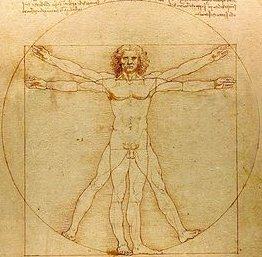
\includegraphics[width=0.35\textwidth]{vitruvio2.jpg}
    \caption{Hombre de Vitruvio, el dibujo más conocido de Leonardo Da Vinci.\cite{RefWorks:71}} % URL:http://upload.wikimedia.org/wikipedia/commons/thumb/2/22/Da_Vinci_Vitruve_Luc_Viatour.jpg/300px-Da_Vinci_Vitruve_Luc_Viatour.jpg  http://commons.wikimedia.org/wiki/File:Da_Vinci_Vitruve_Luc_Viatour.jpg#mediaviewer/Archivo:Da_Vinci_Vitruve_Luc_Viatour.jpg
\end{figure}

\section{Andrés Vesalio} \label{app:vesalio}

Andrés Vesalio fue un pionero en el ámbito de la anatomía. En su tratado ``De humani corporis fabrica'' se pueden apreciar diversas representaciones de la anatomía del cuerpo humano en movimiento. A continuación están detallados algunos de estos dibujos:
\begin{figure}[H]
    \centering
        \begin{subfigure}[b]{0.26\textwidth}
             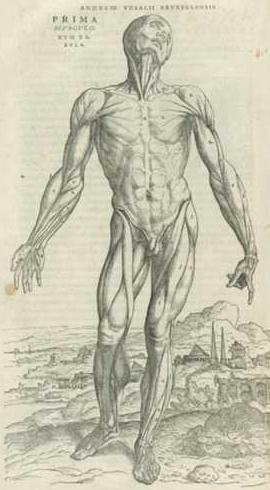
\includegraphics[height=6cm]{musculos.jpg}
             \caption{Músculos\cite{RefWorks:41}}
        \end{subfigure}
        \begin{subfigure}[b]{0.26\textwidth}
             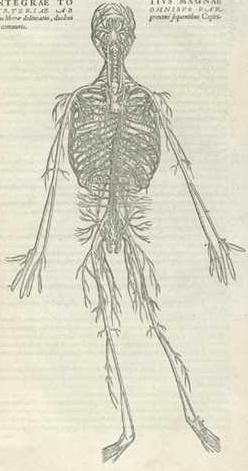
\includegraphics[height=6cm]{nervios.jpg}
             \caption{Nervios\cite{RefWorks:41}}
        \end{subfigure}
        \begin{subfigure}[b]{0.26\textwidth}
            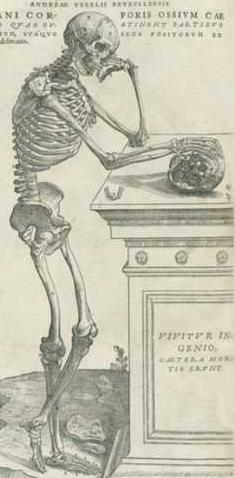
\includegraphics[height=6cm]{esqueleto.jpg}
            \caption{Esqueleto\cite{RefWorks:41}}
        \end{subfigure}
        \begin{subfigure}[b]{0.35\textwidth}
             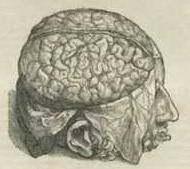
\includegraphics[width=\textwidth]{cabeza.jpg}
             \caption{Cabeza y cerebro\cite{RefWorks:41}}
        \end{subfigure}
        \begin{subfigure}[b]{0.28\textwidth}
             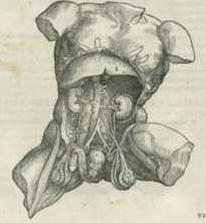
\includegraphics[width=\textwidth]{interior.jpg}
             \caption{Órganos internos\cite{RefWorks:41}}
        \end{subfigure}
\end{figure}
% http://www.biografiasyvidas.com/biografia/v/vesalio.htm
% http://archive.nlm.nih.gov/proj/ttp/flash/vesalius/vesalius.html
% http://quod.lib.umich.edu/w/wantz/vesd1.htm
% Andrés Vesalio, su vida y su obra Escrito por José Barón Fernández

\section{Tipos de Cruces} \label{app:crosses}

Tradicionalmente existen cuatro tipos de cruces según su morfología específica básica. Estos cuatro modelos son:
%\begin{itemize}
%\item[La cruz Latina, cruz immissa o cruz ordinaria]
%\item[La cruz Griega o cruz immissa quadrata]
%\item[La cruz de San Andrés o cruz decussata]
%\item[La cruz Tau, cruz commissa o en forma de T]
%\end{itemize}

\begin{description}
\item[] La cruz Latina, cruz \textit{Immissa} o cruz ordinaria
\item[] La cruz Griega o cruz \textit{Immissa quadrata}
\item[] La cruz de San Andrés o cruz \textit{Decussata}
\item[] La cruz Tau, cruz \textit{Commissa} o en forma de T
\end{description}


\begin{figure}[H]
    \centering
    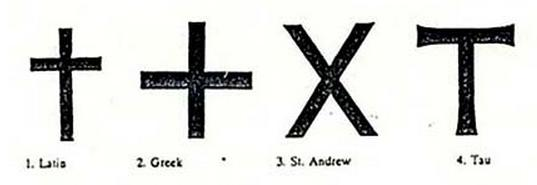
\includegraphics[width=1\textwidth]{cruces.jpg}
    \caption{Distintos tipos de cruces.\cite{RefWorks:43}} % URL:http://www.crosses.org/history.htm
\end{figure}

\section{Cristo de San Juan de la Cruz} \label{app:sanjuan}

\begin{figure}[H]
    \centering
    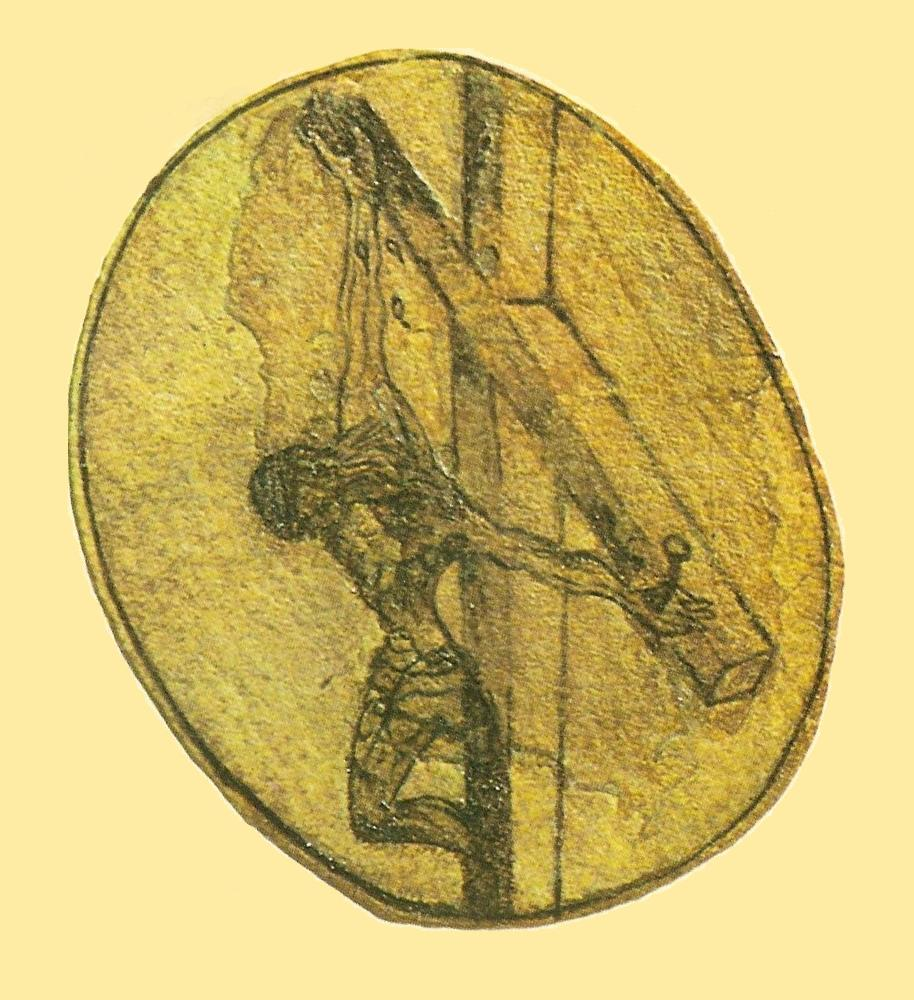
\includegraphics[width=0.55\textwidth]{sanju.jpg}
    \caption{Cristo original de San Juan de la Cruz, que inspiró a Dalí en su obra.\cite{RefWorks:44}} % URL:http://archipielagoduda.blogspot.com.es/2011/03/el-unico-dibujo-conservado-de-san-juan.html
\end{figure}

\section{Cristo Crucificado de la Hermandad Universitaria de Córdoba} \label{app:crucificadominarro}

Este Cristo crucificado realizado por Juan Manuel Miñarro se encuentra en la Hermandad Universitaria de Córdoba y sirve de paso de semana santa en las procesiones de esta ciudad.

\begin{figure}[H]
    \centering
    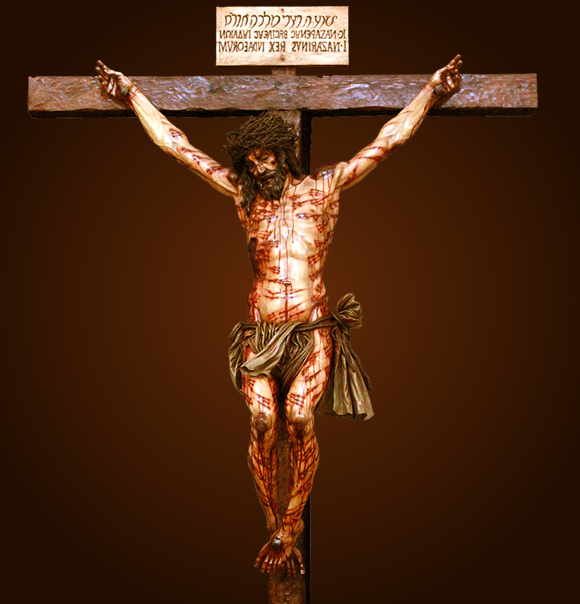
\includegraphics[width=0.58\textwidth]{crucificadominarro.jpg}
    \caption{Escultura de Cristo crucificado realizada por Miñarro.\cite{RefWorks:70}} % URL: http://hermandaduniversitaria.files.wordpress.com/2012/04/sesion5_big.jpg
\end{figure}

\section{La Síndone de Turín o Sábana Santa} \label{app:sindone}

\begin{figure}[H]
    \centering
    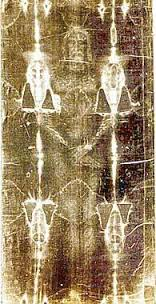
\includegraphics[width=0.27\textwidth]{sindone.jpg}
    \caption{Tela de lino que posee grabada la imagen de un hombre con marcas de martirio y crucifixión. Se cree que pudo envolver a Cristo tras su muerte.\cite{RefWorks:72}} % URL:http://www.lanuovaregaldi.it/photo/eventi/sindonetorino.jpg
\end{figure}

